\documentclass[a4paper,10pt]{article}

\usepackage[spanish, activeacute]{babel}
\usepackage{a4wide}
\usepackage{enumerate}
\usepackage[utf8]{inputenc}
\usepackage{graphicx}
\usepackage{multicol}
\usepackage{multirow}
\usepackage{latexsym}


\usepackage{listings}
\lstdefinestyle{C}
   {language=C,frame=Ltb,
     framerule=0pt,
     %aboveskip=0.5cm,
     %framextopmargin=3pt,
     %framexbottommargin=3pt,
     %framexleftmargin=0.4cm,
     framesep=0pt,
     rulesep=.4pt,
     backgroundcolor=\color{gris95},
     rulesepcolor=\color{black},
     %
     stringstyle=\ttfamily,
     showstringspaces = false,
     basicstyle=\small\ttfamily,
     commentstyle=\color{gray45},
     keywordstyle=\bfseries,
     %
     numbers=left,
     numbersep=1em,
     numberstyle=\tiny,
     numberfirstline = false,
     breaklines=true,
   }


\addtolength\topmargin{-1cm}
\setlength\voffset{0cm}
\setlength\headheight{0cm}
\setlength\headsep{0cm}
\addtolength\textheight{4cm}

\title{TCP - Control de Congestion}
\author{Según RFC 2581}
\date{}

\def\ack{\texttt{ACK}\ }
\newcommand\cmd[1]{\texttt{#1}}
\begin{document}
\maketitle

\section*{Esquema de transiciones}

\scalebox{0.6}{
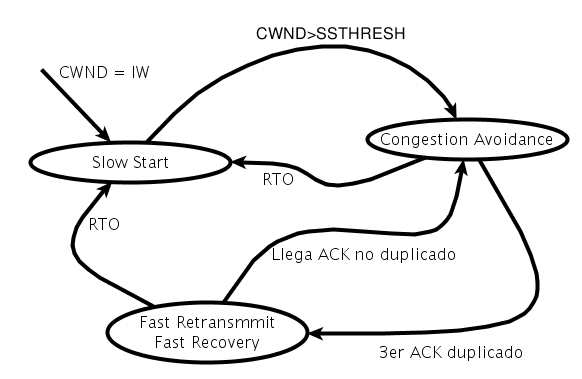
\includegraphics[scale=1]{TCP.png}
}

\section*{Comentarios globales}
\begin{itemize}
	\item Sólo se puede enviar \texttt{min (CWND, RWND)}.
	\item Datos variables: \cmd{CWND RWND SSTRESH}
	\item Constantes: \cmd{IW LW SMSS}
	\item Datos que cambian pero que no nombramos acá: \cmd{RTO}
\end{itemize}


\section*{Slow Start}
Se usa cuando se inicia la transmisión o luego de un \cmd{RTO}. El mismo
implica:
\begin{itemize}
	\item \cmd{IW <= 2 * SMSS}
	\item Si es al comienzo de la conexión: \cmd{CWND = IW}, si proviene de un
		\cmd{RTO} entonces \cmd{CWND = LW}, que \cmd{LW = 1}.
	\item Por cada \ack recibido \cmd{CWND = 2 * CWND}
	\item Pasa a \emph{Congestion Avoidance} cuando \cmd{CWND > SSTRESH}		
\end{itemize}
Inicialmente el \cmd{SSTRESH} debe tener un valor muy grande para explorar la
red, un buen valor podría ser \cmd{RMWND}.

\section*{Congestion Avoidance}
Este algoritmo implica:
\begin{itemize}
	\item Por cada \ack recibido \cmd{CWND += SMSS*SMSS/CWND}, si da menos que
		1, suma 1.
	\item Pasa a \emph{Fast Retransmit/Fast Recovery} cuando hay 3 \ack s duplicados
	\item Pasa a \emph{Slow Start} luego de un \cmd{RTO} y en ese caso se
		modifica el \cmd{SSTRESH}\\ 
		\cmd{SSTRESH = max(''datos en vuelo''/2, 2 * SMSS)}
\end{itemize}

\section*{Fast Retransmit/Fast Recovery}
Cuando el emisor recibe el tercer \ack duplicado, este envía el segmento primer
segmento del cual no recibió \ack y pasa a \emph{Fast Recovery}. Para que esto
funcione bien, el receptor no debe retrasar los \ack de los segmentos que no
llegan en orden.

Hace lo siguiente:

\begin{enumerate}[i.]
	\item 	Cuando recibe el tercer \ack duplicado cambia del \cmd{SSTRESH} a uno
		que cumpla que \\ \cmd{SSTRESH <= max(''datos en vuelo''/2, 2 * SMSS)}
	\item	Retransmite el segmento del cual no recibió \ack y cambia a:
		\cmd{CWND = SSTRESH + 3 * SMSS}
	\item 	Por cada \ack duplicado extra que reciba incrementa \cmd{CWND += 1
		SMSS}
	\item Si \cmd{CWND} y \cmd{RWND} lo permiten, transmite un nuevo segmento.
	\item Termina cuando:
		\begin{enumerate}
			\item Recibe un \ack no duplicado. Lo cual provoca un cambio en
				\cmd{CWND = SSTRESH} y que pase a \emph{Congestion Avoidance}
			\item Ocurre el \cmd{RTO} y vuelve a \emph{Slow Start} con
				\cmd{CWND=IW}
		\end{enumerate}
\end{enumerate}

\section*{Glosario}
\begin{description}
	\item[CWND] Congestion Window
	\item[IW]	Initial Window
	\item[LW]	Loss Window
	\item[RTO]	Retransmission TimeOut
	\item[RWND] Receiver Window
	\item[SMSS]	Sender Maximum Segment Size
	\item[SSTRESH] Slow Start Treshold

\end{description}

\end{document}
